%% question-6.tex
%%

%% ==============================
\subsection{Diagramme d'objet d'un monde}
\label{sec:question-6}
%% ==============================

Le diagramme d'objet suivant décrit le monde de taille 4:

\begin{figure}
	\centering
	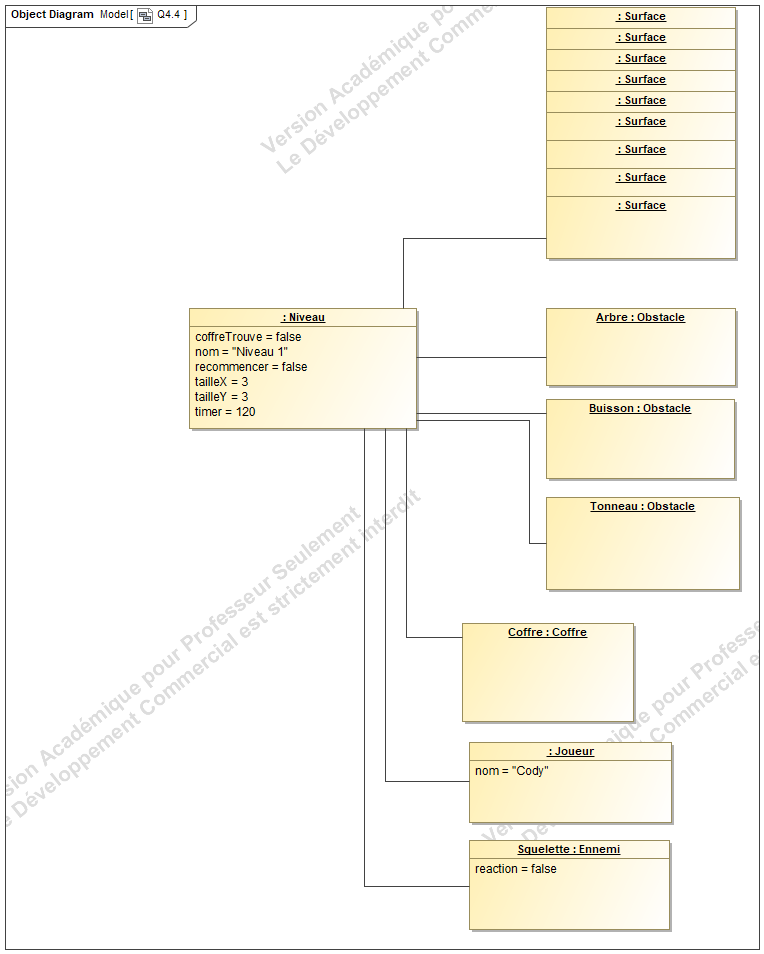
\includegraphics[width=\textwidth]{assets/Diagramme_objet}
	\caption{Diagramme d'objet}
	\label{fig:diagrammeobjet}
\end{figure}